
\noindent \textbf{Why study abelian gauge theory?}

\noindent An example of an abelian gauge theory is quantum electrodynamics and the electromagnetic field, as well as $SU(2)$, and $SU(3)$ gauge bosons. \\

\noindent In developing a gauge theory, we will follow the same route of specifying symmetries, giving rise to invariants, of the theory and then, via quantization, look for (projective) unitary representations of the group which are local. \\

\noindent As opposed to other field theories, the gauge theory should be symmetric under a local gauge group $\mathcal{G}$ which acts independently at each location in spacetime. \\

\noindent For example, consider the circle group $U(1)$, which consists of all complex numbers with absolute value equal to 1 under multiplication, the roots of unity

\begin{equation}
U(1) = \{ e^{i \theta} : \, \theta \in [0, 2 \pi ) \}.
\end{equation}

\noindent This symmetry group gives rise to the local gauge group $\mathcal{G}$ as the group of transformations from $1+3$-dimensional space time, Minkowski space, to the circle group

\begin{equation}
\mathcal{G} = \{ g: \,\, \mathcal{M}_{1+3} \rightarrow U(1) \}
\end{equation}

\noindent \textbf{How does the local gauge group act on fields? }\\

\noindent Consider the DIrac field, where we want a $U(1)$ gauge-invariant quantum field theory of electrons. Elements of $\mathcal{G}$ act independently on each spacetime location$x \in \mathcal{M}_{1+3}$. Equivalently, there is a copy of $U(1)$ attached to each $x$ acting independently of each other.

\begin{equation}
g: \, \psi (x) \rightarrow \pi ( g (x) ) \psi(x) = e^{i \alpha (x)} \psi (x)
\end{equation}

\noindent Where $\theta(x) \in [ 0 , 2 \pi )$ is a phase factor. \\

\noindent \textbf{Which theories are invariant under the Poincar\'e group and the local gauge group $\mathcal{G}$?} \\

\noindent As it stands, we have an empty set of theories that are invariant under the local gauge group. Begin populating it by building a Lagrangian density, with a classical, continuous spacetime, and find which kinds of terms will be invariant. \\

\noindent Terms of the Lagrangian density for the Dirac field that we already know to be invariant are $\bar{\psi}\psi$ and $(\bar{\psi} \gamma^/mu \psi)^2$ (contracted with itself). \\

\noindent Note that the quantity $\bar{\psi} \slashed{\partial} \psi$ is not invariant, as it is not well-defined!  Why? \\

\noindent The differential operator acting on the field $\partial_\mu \psi$ is a limit

\begin{equation}
\partial_\mu \psi \equiv \lim_{\epsilon \rightarrow \infty} \frac{ \psi(x + \epsilon n^\mu) - \psi(x)}{\epsilon}.
\end{equation}

\noindent And the local gauge group acting on this quantity results in oscillatory terms that do not converge as $\epsilon \rightarrow 0$ (e.g., $\sim e^{i\dots}$). The limit does exist under gauge transformations, since

\begin{equation}
g(\partial_\mu \psi) = \lim_{\epsilon \rightarrow \infty} \frac{1}{\epsilon} (e^{- \theta(x + \epsilon n^\mu)} \psi(x + \epsilon n^\mu ) - e^{i \theta(x)} \psi (x) ).
\end{equation}

\noindent This theory is boring at this moment, as the Lagrangian has only two gauge-invariant terms. To introduce dynamics and impose the desired symmetry, we need the derivative, but there is no way to do it with a single fermion (or boson) field. Therefore, we introduce an \textit{auxiliary field} which transforms nontrivially on the local gauge group (c.f., adding a catalyst in chemistry opens new thermodynamic paths for reactions to take place, as the catalyst is not consumed, but is used, in the reaction to lowers the free energy of the reaction). \\

\noindent Introduce the \textit{parallel transporter}, a recipe to compare a field at two independent spacetime locations, which is dependent on the path $\gamma$

\begin{equation}
U_\gamma (y,x) \in U(1), \,\, \forall \, x, y \in \mathcal{M}_{1+3}
\end{equation}

\noindent To ensure that $U(y,x)$ is a gauge invariant comparator, and allow us to compare the two spacetime locations in a gauge invariant, we require that the local gauage group act as

\begin{equation}
g: \,\, U(y,x) \rightarrow e^{i \alpha (y)} U(y,x) e^{-i \theta(x)}.
\end{equation}

\noindent So, we define $\psi(x)$ to be \textit{parallel transported} to $y$ as

\begin{align}
g: \,\, U(y,x) \psi(x) &\rightarrow e^{i \theta(y)} U(y,x) e^{-i \theta(x) }e^{- \alpha (x)} \psi(x) \\
&= e^{i \theta(y)} U(y,x)  \psi(x)
\end{align}

\noindent \textbf{Does such an object $U(y,x)$ exist?} \\

\noindent Yes, they exist and are made rigorous in the formalism of fibre bundles and principal bundles. Note that $U(y,x)$ is a not a field and is nonlocal object, but it is expressable in terms of local objects and local data. \\

\noindent So, $\psi(x + \epsilon n^\mu)$ and $U(x+\epsilon n^\mu, x)\psi(x)$ transform the same way under the local gauge group $\mathcal{G}$, and we can introduce dynamics to the theory and define the \textit{covariant derivative} as

\begin{equation}
D_\mu \psi (x) \equiv \lim_{\epsilon \rightarrow 0} \frac{\psi (x + \epsilon n^\mu) - U (x + \epsilon n^\mu, x) \psi (x)}{\epsilon}
\end{equation}

\noindent \textbf{What about the parallel transporter $U(y,x)$?} \\

\noindent Suppose that $U(x + \epsilon n^\mu , x)$ is continuous and differentiable near $x$, and apply the Taylor series expansion

\begin{align}
U(x + \epsilon n^\mu , x) &= U (x,x) + \epsilon n^\mu \partial_\mu U(x,x) + \dots \\
&= 1 + \epsilon n^\mu \partial_\mu U(x,x) +\dots \\
&= 1 - i \epsilon n^\mu A_\mu (x) + \dots
\end{align}

\noindent Where we tried $U(x,x)=1$, since $1$ transforms correctly under the gauge group, and it is traditional to call $\partial_\mu U(x,x) = -i \alpha A_\mu (x)$, where $\alpha$ is the fine structure constant. Now, $A_\mu (x)$ is not arbitrary, and must satisfy some constraints. \\

\noindent \textbf{How does $A_\mu (x)$ transform under $\mathcal{G}$?} \\

\noindent Apply a local gauge transformation $g \in \mathcal{G}$ to the last line above

\begin{equation}
e^{i \alpha (x + \epsilon n^\mu)} U(x + \epsilon n^\mu, x) e^{-i \theta(x)} = 1 - i \alpha \epsilon n^\mu A_\mu (x) + i n^\mu \partial_\mu \theta(x) + \dots
\end{equation}

\noindent Thus, the auxiliary field transforms under the local gauge as

\begin{equation}
g: \,\, A_\mu (x) \rightarrow A_\mu (x) - \frac{1}{\alpha} \partial_\mu \theta (x)
\end{equation}

\noindent And this gives us a definition of $A_\mu (x)$ in one gauge, and this transformation law allows us to change gauge, or basis. Finding the form of $A_\mu (x)$ that satisfies this local gauge transformation is tantamount to having an infinitesimal method for building the parallel transporter object. \\

\noindent Put this all together into the covariant derivative (\textbf{Exercise})

\begin{equation}
D_\mu \psi (x) = \partial_\mu \psi (x) + i \alpha A_\mu (x) \psi (x)
\end{equation}

\noindent Which is now a purely local object, dependent on only one spacetime location $x$. \\

\noindent Furthermore, the covariant derivative of the field transforms under the local gauge group by introducing the phase factor, the same as the action of $\mathcal{G}$ on the field $\psi$ itself

\begin{equation}
g: \,\, D_\mu \psi (x) \rightarrow e^{i \alpha (x)} D_\mu \psi (x)
\end{equation}

\noindent So, we've built the parallel transporter in terms of the local field $A_\mu (x)$, and we have a derivative object that transforms correctly under the local gauge group. Now, build the Lagrangian density

\begin{equation}
\mathcal{L} = \bar{\psi} \slashed{D} \psi - m \bar{\psi} \psi + \text{auxiliary field term(s)}
\end{equation}

\noindent To include the auxiliary field $A_\mu (x)$ in the quantization we need to endow it with dynamics. \\

\noindent \textbf{How do we give $A_\mu (x)$ dynamics?} \\

\noindent To first order,

\begin{equation}
U(x+\epsilon n^\mu , x) \sim e^{-i\alpha \epsilon n^\mu A_\mu (x + \frac{1}{2} \epsilon n^\mu)}.
\end{equation}

\noindent Use the parallel transporter to build a \textit{plaquette operator}, which transverses an object around a square of dimension $\epsilon$

\begin{figure}[H]
	\centering
	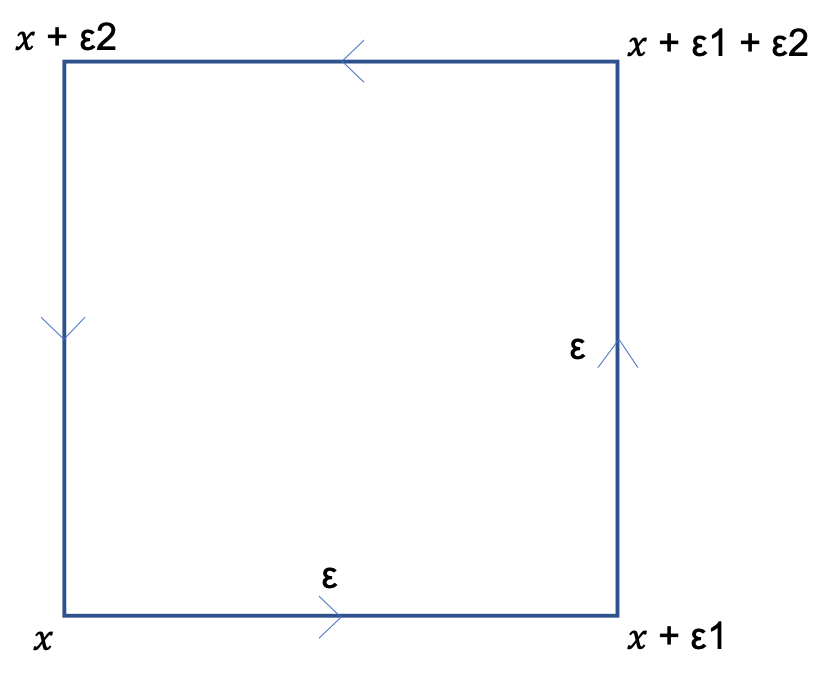
\includegraphics[width=2in]{images/plaquette.png}
\end{figure}

\begin{equation}
U_\Box(x)  = U(x, x + \epsilon \hat{1}) \cdot U (x + \epsilon \hat{1}, x + \epsilon (\hat{1} + \hat{2})) \cdot U(x + \epsilon (\hat{1} + \hat{2}), x + \epsilon \hat{2}) \cdot U(x + \epsilon \hat{2}, x).
\end{equation}

\noindent The plaquette operator $U_\Box$ is gauge invariant, and, working out the Taylor series, we can write it in terms of the auxiliary field (\textbf{Exercise})

\begin{equation}
U_\Box (x)  = e^{-i \epsilon \alpha (-A_2 (x + \frac{1}{2} \epsilon \hat{2}) - A_1 (x + \frac{1}{2} \epsilon \hat{1} + \epsilon \hat{2}) + A_2 (x + \epsilon \hat{1} +\frac{1}{2} \epsilon \hat{2}) + A_1 (x + \frac{1}{2} \epsilon \hat{1})) + \mathcal{O} (\epsilon^3)}.
\end{equation}

\noindent Expand in $\epsilon$ (\textbf{Exercise})

\begin{equation}
U_\Box (x) = 1 - i \epsilon^2 \alpha (\partial_1 A_2 - \partial_2 A_1 ) + \mathcal{O} (\epsilon^3).
\end{equation}

\noindent The choice of direction in this derivation is arbitrary, leaving 16 possible choices; construct the 2-tensor

\begin{equation}
F_{\mu\nu} (x) = \partial_\mu A_\nu - \partial_\nu A_\mu.
\end{equation}

\noindent Note that $F_{\mu\nu}$ is locally gauge invariant, Lorentz invariant, but it is not Poincar\'e invariant with those spacetime indices. Construct the gauge, Lorentz, and Poincar\'e invariant object from the $F_{\mu\nu}$

\begin{equation}
-\frac{1}{4} F^{\mu\nu} F_{\mu\nu}.
\end{equation}

\noindent Then the first nontrivial Langrangian density we can construct is the exact Lagrangian for quantum electrodynamics: an electromagnetic field minimally coupled to the Dirac field.

\begin{equation}
\mathcal{L} = \bar{\psi} (\slashed{D} - m) \psi -\frac{1}{4} F^{\mu\nu} F_{\mu\nu}.
\end{equation}

\noindent The term ``minimally coupled'' means that the theory is renormalizable. \\

\subsection*{Alternative Derivation of $F^{\mu\nu}$}

\noindent Since $D_\mu$ is gauage invariant, the commutator with itself $[D_\mu, D_\nu ]$ is also gauge invariant. So, under the local gauge group, the commutator transforms as

\begin{equation}
g: \,\, [D_\mu, D_\nu] \psi (x) \rightarrow e^{i \alpha (x)} [D_\mu, D_\nu] \psi (x).
\end{equation}

\noindent Plugging in the expression for the covariant derivative and working out the commutator, we get

\begin{equation}
[D_\mu, D_\nu] \psi (x) = [\partial_\mu, \partial_\nu] \psi + i \alpha ( [\partial_\mu, A_\nu] - [\partial_\nu, A_\mu]) \psi - \alpha^2 [A_\mu, A_\nu] \psi.
\end{equation}

\noindent The commutators of $\partial$ and $A$ with themselves are zero. Therefore,

\begin{equation}
[D_\mu, D_\nu] \psi (x) = i \alpha ( \partial_\mu A_\nu - \partial_\nu A_\mu) \psi (x)
\end{equation}

\noindent The commutator of the covariant derivative is the \textit{spacetime curvature tensor}.

\begin{equation}
[D_\mu, D_\nu] \psi (x) =i \alpha F_{\mu\nu} (x).
\end{equation}